\input cwebmac
\documentclass{cweb}
\usepackage{geometry}
\usepackage{amsmath,amssymb}
\usepackage{mathtools}
\usepackage{physics}
\usepackage{graphicx}

\geometry{a4paper,centering,scale=0.8}

\bibliographystyle{plain}

\begin{document}

\title{A Program to Calculate Chiral Charge Separation in Heavy-Ion Collisions}
\author{Ai Xin}

\maketitle


\N{1}{1}Introduction.

This is a program to calculate Chiral Charge Separation in Heavy-Ion
Collisions.
Here is an overview of the structure of the program:
\Y\B\X2:Header files to include\X\6
\X3:Function prototype\X\6
\X5:Global variables\X\6
\X4:Function: square and cube\X\6
\X7:Function: number density of nuclei\X\6
\X8:Function: rapidity distribution of ``participants''\X\6
\X12:Function: ``participants'' integrand function\X\6
\X13:Function: ``spectators'' integrand function\X\6
\X14:Function: calculate magetic field\X\6
\X21:Function: convert collision energy to rapidity\X\6
\X16:Function: $\xi_\pm$ function\X\6
\X17:Function: $\langle \Delta_\pm^2 \rangle$ integrand function\X\6
\X18:Function: $\langle \Delta_+ \Delta_- \rangle$ integrand function\X\6
\X19:Function: calculate chiral separation effects\X\6
\X20:The main program\X\par
\fi

\M{2}This program obviously need include the standard I/O library. It also need
GSL math library and the standard math library. Finally, we need Cuba library
to do integration.
\Y\B\4\X2:Header files to include\X${}\E{}$\6
\8\#\&{include} \.{<stdio.h>}\6
\8\#\&{include} \.{<stdlib.h>}\6
\8\#\&{include} \.{<gsl/gsl\_math.h>}\6
\8\#\&{include} \.{<math.h>}\6
\8\#\&{include} \.{<string.h>}\6
\8\#\&{include} \.{<cuba.h>}\par
\U1.\fi

\M{3}Now we define function prototype.
\Y\B\4\X3:Function prototype\X${}\E{}$\6
\&{double} \\{Sq}(\&{double} \\{num});\6
\&{double} \\{Pow3}(\&{double} \\{num});\6
\&{double} \\{rhoFun}(\&{double} \\{xp}${},\39{}$\&{double} \\{yp}${},\39{}$%
\&{double} \\{zp});\6
\&{double} \|f(\&{double} \|Y);\6
\&{static} \&{int} \\{eB\_Part\_Int}(\&{const} \&{int} ${}{*}\\{ndim},\39{}$%
\&{const} \&{double} \\{xx}[\,]${},\39{}$\&{const} \&{int} ${}{*}\\{ncomp},%
\39{}$\&{double} \\{ff}[\,]${},\39{}$\&{void} ${}{*}\\{userdata});{}$\6
\&{static} \&{int} \\{eB\_Spec\_Int}(\&{const} \&{int} ${}{*}\\{ndim},\39{}$%
\&{const} \&{double} \\{xx}[\,]${},\39{}$\&{const} \&{int} ${}{*}\\{ncomp},%
\39{}$\&{double} \\{ff}[\,]${},\39{}$\&{void} ${}{*}\\{userdata});{}$\6
\&{int} \\{eB}(\&{double} ${}{*}\\{eBy},\39{}$\&{double} ${}{*}\\{totalerror},%
\39{}$\&{const} \&{int} \\{verbose});\6
\&{double} \\{xifun}(\&{double} \\{xp}${},\39{}$\&{double} \\{yp}${},\39{}$%
\&{char} \\{sign});\6
\&{static} \&{int} \\{delta\_pp\_Int}(\&{const} \&{int} ${}{*}\\{ndim},\39{}$%
\&{const} \&{double} \\{xx}[\,]${},\39{}$\&{const} \&{int} ${}{*}\\{ncomp},%
\39{}$\&{double} \\{ff}[\,]${},\39{}$\&{void} ${}{*}\\{userdata});{}$\6
\&{static} \&{int} \\{delta\_pm\_Int}(\&{const} \&{int} ${}{*}\\{ndim},\39{}$%
\&{const} \&{double} \\{xx}[\,]${},\39{}$\&{const} \&{int} ${}{*}\\{ncomp},%
\39{}$\&{double} \\{ff}[\,]${},\39{}$\&{void} ${}{*}\\{userdata});{}$\6
\&{int} \\{csefun}(\&{double} ${}{*}\\{app},\39{}$\&{double} ${}{*}\\{apm},%
\39{}$\&{double} ${}{*}\\{delta\_pp},\39{}$\&{double} ${}{*}\\{delta\_pm});{}$\6
\&{int} \\{main}(\&{int} \\{argc}${},\39{}$\&{char} ${}{*}{*}\\{argv});{}$\6
\&{double} \\{sqrtStoY}(\&{double} \\{sqrtS});\par
\U1.\fi

\M{4}To speed up the calculation processes, we define inline function of square
and cube.
\Y\B\4\X4:Function: square and cube\X${}\E{}$\6
\&{double} \\{Sq}(\&{double} \\{num})\1\1\2\2\6
${}\{{}$\1\6
\&{return} \\{num}${}*\\{num};{}$\6
\4${}\}{}$\2\7
\&{double} \\{Pow3}(\&{double} \\{num})\1\1\2\2\6
${}\{{}$\1\6
\&{return} \\{num}${}*\\{num}*\\{num};{}$\6
\4${}\}{}$\2\par
\U1.\fi

\M{5}For convenience, we define some global variables.
\Y\B\4\X5:Global variables\X${}\E{}$\6
\&{static} \&{const} \&{double} \\{alpha\_EM}${}\K\T{1.0}/\T{137.0};{}$\6
\&{static} \&{const} \&{double} \\{hbarc}${}\K\T{197.32696};{}$\6
\&{static} \&{double} \|R;\SHC{ radius of the nucleus }\6
\&{static} \&{double} \|b;\SHC{ impact parameter }\6
\&{static} \&{double} \|d;\SHC{ geometry distribution factor of the nucleus }\6
\&{static} \&{double} \\{n0};\SHC{ central number density of the nucleus }\6
\&{static} \&{double} \.{Y0};\SHC{ initial rapidity }\6
\&{static} \&{double} \|t;\SHC{ time }\6
\&{static} \&{double} \\{t0};\6
\&{static} \&{double} \\{eBy0};\6
\&{static} \&{double} \|x${},{}$ \|y${},{}$ \|z;\SHC{ field point coordinates }%
\6
\&{static} \&{double} \|Z;\6
\&{static} \&{double} \|a;\6
\&{static} \&{char} \\{flag};\SHC{ '+' or '-', denote left or right nucleus }\6
\&{static} \&{double} \\{lambda};\SHC{ screening length }\6
\&{static} \&{double} \\{Np}${},{}$ \\{Nm};\7
\&{static} \&{int} \\{nvec}${}\K\T{1};{}$\6
\&{static} \&{double} \\{epsrel};\6
\&{static} \&{double} \\{epsabs};\6
\&{static} \&{int} \\{flags};\6
\&{static} \&{int} \\{seed};\6
\&{static} \&{int} \\{pmineval};\6
\&{static} \&{int} \\{pmaxeval};\6
\&{static} \&{int} \\{smineval};\6
\&{static} \&{int} \\{smaxeval};\6
\&{static} \&{int} \\{mineval};\6
\&{static} \&{int} \\{maxeval};\6
\&{static} \&{int} \\{nstart};\SHC{ [V]the number of integrand evaluations per
iteration to start with. demo's value is 1000 }\6
\&{static} \&{int} \\{nincrease};\SHC{ [V]the increase in the number of
integrand evaluations per iteration. demo's value is 500 }\6
\&{static} \&{int} \\{nbatch};\SHC{ [V]the batch size for sampling. demo's
value is 1000 }\6
\&{static} \&{int} \\{gridno};\SHC{ [V]the slot in the internal grid table.
demo's value is 0 }\6
\&{static} \&{int} \\{nnew};\SHC{ [S]the number of new integrand evaluations in
each subdivision. demo's value is 1000 }\6
\&{static} \&{int} \\{nmin};\SHC{ [S]the minimum number of samples a former
pass must contribute }\SHC{ to a subregion to be considered in that region’s
compound integral value. demo's value is 2. }\6
\&{static} \&{double} \\{flatness};\SHC{ [S]the parameter p in Eq. (1). demo's
value is 25. }\6
\&{static} \&{int} \\{key1};\SHC{ [D]determines sampling in the partitioning
phase. demo's value is 47 }\6
\&{static} \&{int} \\{key2};\SHC{ [D]determines sampling in the final
integration phase. demo's value is 1 }\6
\&{static} \&{int} \\{key3};\SHC{ [D]sets the strategy for the refinement
phase. demo's value is 1 }\6
\&{static} \&{int} \\{maxpass};\SHC{ [D]controls the thoroughness of the
partitioning phase. demo's value is 5. }\6
\&{static} \&{double} \\{border};\SHC{ [D]the width of the border of the
integration region. demo's value is 0. }\6
\&{static} \&{double} \\{maxchisq};\SHC{ [D]the maximum χ 2 value a single
subregion is allowed to have in the final integration phase. demo's value is
10. }\6
\&{static} \&{double} \\{mindeviation};\SHC{ [D]a bound, given as the fraction
of the requested error of the entire integral. demo's value is 0.25. }\6
\&{static} \&{int} \\{ngiven};\SHC{ [D]the number of points in the xgiven
array. demo's 0 }\6
\&{static} \&{int} \\{ldxgiven};\SHC{ [D]the leading dimension of xgiven, i.e.
the offset between one point and the next in memory. demo's value is NDIM }\6
\&{static} \&{int} \\{nextra};\SHC{ [D]the maximum number of extra points the
peak-finder subroutine will return. demo's value is 0. }\6
\&{static} \&{int} \\{key};\SHC{ [C]chooses the basic integration rule. demo's
value is 0 }\6
\&{static} \&{char} ${}{*}\\{statefile};{}$\6
\&{static} \&{void} ${}{*}\\{spin}{}$;\SHC{ the ‘spinning cores’ pointer,
demo's value is NULL }\par
\U1.\fi

\M{6}Let's first consider the magnetic field produced by a point charge.
Namely, the magnetic field at position $\vb*{x} = (\vb*{x}_\perp , z)$ caused
by a particle with charge $Z$ moving in the positive $z$-direction with
rapidity $Y$. At $t = 0$ the particle can be found at position $\vb*{x}'_%
\perp$. The result is
\begin{equation}
e\vb*{B}(\vb*{x}) = Z \alpha_{\text{EM}} \sinh(Y) \frac{(\vb*{x}'_\perp - %
\vb*{x}_\perp) \times \vb*{e}_z}{[(\vb*{x}'_\perp - \vb*{x}_\perp)^2 + (t\sinh
Y - z \cosh Y)^2]^{3/2}}.
\end{equation}

For heavy-ion collisions, we set the nuclei completely collided at $t = 0$,
where their center is at point $(\pm\vb*{b}/2,0)$ as in figure \ref{fig01}. We
can then split the total magnetic field in the following way
\begin{equation}
\vb*{B} = \vb*{B}_s^+ + \vb*{B}_s^- + \vb*{B}_p^+ + \vb*{B}_p^-.
\end{equation}
where $\vb*{B}_s^\pm$ and $\vb*{B}_p^\pm$ are the contributions of the
``spectators'' and ``participants''. To calculate it, we need the phase
configuration of the charged particles, namely it's position distribution and
rapidity distribution.

\begin{figure}
\centering
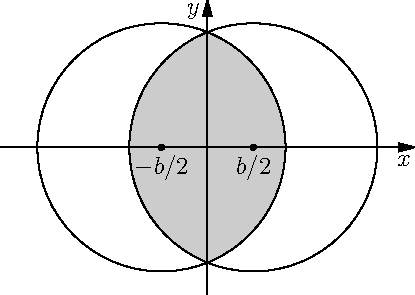
\includegraphics[scale=1]{fig1}\\
\caption{Cross section of peripheral collision, where the shadow part denotes
``participants'' and the other part denotes ``spectators''. The left nucleus
moves along the positive $z$ direction, while the right nucleus moves along the
negative $z$ direction. The $z$ direction is outwardly perpendicular to the
paper.}\label{fig01}
\end{figure}

\fi

\M{7}When a nucleus stays at rest, its nucleus number density distribution can
be discribed by Woods-Saxon distribution
\begin{equation}
n_A(r) = \frac{n_0}{1 + \exp(\frac{r-R}{d})}.
\end{equation}
This distribution must be modified due to the Lorentz contraction of the
nuclei, so we have
\begin{equation}
\rho_\pm (\vb*{x}') = \frac{\gamma n_0}{1 + \exp(\frac{\sqrt{(x'\pm b/2)^2 +
y'^2 + (\gamma z')^2} - R}{d})}.
\end{equation}
where the subscript $+(-)$ denotes the left(right) nucleus moving along the
positive(negative) $z$ direction, $\gamma$ is the Lorentz contraction factor.
Here we define a function to calculate the number density of the nuclei.

\Y\B\4\X7:Function: number density of nuclei\X${}\E{}$\6
\&{double} \\{rhoFun}(\&{double} \\{xp}${},\39{}$\&{double} \\{yp}${},\39{}$%
\&{double} \\{zp})\1\1\2\2\6
${}\{{}$\SHC{ \PB{\\{xp}}, \PB{\\{yp}}, \PB{\\{zp}}: source point coordinates }%
\SHC{ return: number density at (\PB{\\{xp}}, \PB{\\{yp}}, \PB{\\{zp}}) }\1\6
\&{double} \\{rho};\6
\&{double} \\{len};\6
\&{double} \\{gamma};\6
\&{double} \\{sign}${}\K\T{1.0};{}$\7
${}\\{gamma}\K\\{cosh}(\.{Y0});{}$\6
\&{if} ${}(\\{flag}\E\.{'+'}){}$\5
${}\{{}$\1\6
${}\\{sign}\K\T{1.0}{}$;\SHC{ left nucleus }\6
\4${}\}{}$\2\6
\&{else} \&{if} ${}(\\{flag}\E\.{'-'}){}$\5
${}\{{}$\1\6
${}\\{sign}\K{-}\T{1.0}{}$;\SHC{ right nucleus }\6
\4${}\}{}$\2\6
\&{else}\5
${}\{{}$\1\6
\\{printf}(\.{"[rhoFun]error:\ nucl}\)\.{eus\ type(flag)\ shoul}\)\.{d\ be\ '+'%
\ or\ '-'\\n"});\6
\4${}\}{}$\2\6
${}\\{len}\K\\{sqrt}(\\{Sq}(\\{xp}+\\{sign}*\|b/\T{2.0})+\\{Sq}(\\{yp})+\\{Sq}(%
\\{gamma}*\\{zp}));{}$\6
${}\\{rho}\K\\{gamma}*\\{n0}/(\T{1.0}+\\{exp}((\\{len}-\|R)/\|d)){}$;\SHC{
times gamma for density is increased }\6
\&{return} \\{rho};\6
\4${}\}{}$\2\par
\U1.\fi

\M{8}Now, we consider the rapidity distribution. For ``spectators'', we assume
that they do not effected by the collision, so they just move with rapidity
$Y_0$. For ``participants'', their rapidity distribution is
\begin{equation}
f(Y) = \frac{a}{2\sinh(aY_0)}\exp(aY),\qquad -Y_0 \leq Y \leq Y_0.
\end{equation}
\Y\B\4\X8:Function: rapidity distribution of ``participants''\X${}\E{}$\6
\&{double} \|f(\&{double} \|Y)\1\1\2\2\6
${}\{{}$\1\6
\&{return} ${}(\|a*\\{exp}(\|a*\|Y))/(\T{2}*\\{sinh}(\|a*\.{Y0}));{}$\6
\4${}\}{}$\2\par
\U1.\fi

\M{9}Now we can deduced the magnetic field produced by ``spectators'':
\begin{equation}
\begin{split}
e\vb*{B}_s^\pm(t,\vb*{x}) &= \pm Z \alpha_{\text{EM}} \sinh Y_0 \int_{V_s^\pm} %
\dd[3]{\vb*{x}'} \rho_\pm (\vb*{x}') \\
&\times \frac{(\vb*{x}'_\perp - \vb*{x}_\perp)\times \vb*{e}_z}{[(\vb*{x}'_%
\perp - \vb*{x}_\perp)^2 + ((\frac{z'}{\tanh Y_0} \pm t)\sinh Y_0 - z\cosh
Y_0)^2]^{3/2}}.
\end{split}
\end{equation}
The magnetic field produced by ``participants'':
\begin{equation}
\begin{split}
e\vb*{B}_p^\pm(t,\vb*{x}) &= \pm Z \alpha_{\text{EM}} \int_{V_p} \dd[3]{%
\vb*{x}'} \int_{-Y_0}^{Y_0} \dd{Y} f(Y) \sinh Y \rho_\pm (\vb*{x}') \\
&\times \frac{(\vb*{x}'_\perp - \vb*{x}_\perp)\times \vb*{e}_z}{[(\vb*{x}'_%
\perp - \vb*{x}_\perp)^2 + ((\frac{z'}{\tanh Y_0} \pm t)\sinh Y - z\cosh
Y)^2]^{3/2}}.
\end{split}
\end{equation}
Notice the difference in denominator with point charge magnetic field formula.
The reason is that in point charge magnetic field formula, we assume the point
charge is at $z=0$ plane when $t=0$, however when two nuclei completely collide
not all charge is precisely at $z=0$ plane. So to use the point charge formula,
we need to offset time in the formula. For positively move nucleus,
\begin{equation}
\begin{split}
t \sinh Y - z \cosh Y \rightarrow &  \left(t + \frac{z'}{\tanh Y_0}\right) %
\sinh Y - z \cosh Y_0 \\
& \left(\frac{z'}{\tanh Y_0} + t\right) \sinh Y - z \cosh Y_0
\end{split}
\end{equation}
For negatively move nucleus,
\begin{equation}
\begin{split}
-t \sinh Y - z \cosh Y \rightarrow & -\left(t - \frac{z'}{\tanh Y_0}\right) %
\sinh Y - z \cosh Y_0 \\
& = \left(\frac{z'}{\tanh Y_0} - t\right) \sinh Y - z \cosh Y_0
\end{split}
\end{equation}

\fi

\M{10}To express the integration more explicitly, for  ``participants'' we have
\begin{equation}
\begin{split}
&e\vb*{B}_p^\pm (t, \vb*{x}) = \pm Z \alpha_{\text{EM}} \int_{b/2-R}^{-b/2+R} %
\dd{x'} \int_{-y_{\text{lim}}(x')}^{y_{\text{lim}}(x')} \dd{y'} \int_{-R/\cosh
Y_0}^{R/\cosh Y_0} \dd{z'} \int_{-Y_0}^{Y_0} \dd{Y} f(Y)  \\
&\qquad \sinh Y \rho_\pm(\vb*{x}') \times \frac{(\vb*{x}'_\perp - \vb*{x}_%
\perp)\times \vb*{e}_z}{[(\vb*{x}'_\perp - \vb*{x}_\perp)^2 + ((\frac{z'}{\tanh
Y_0} \pm t)\sinh Y - z\cosh Y)^2]^{3/2}}.
\end{split}
\end{equation}
where $y_{\text{lim}}(x') = \sqrt{R^2 - (^^7c x' ^^7c + b/2)^2}$.

For ``spectators'', it's better to use cylindrical coordinate system.
\begin{equation}
\begin{split}
&e\vb*{B}_s^\pm (t,\vb*{x}) = \pm Z \alpha_{\text{EM}} \sinh Y_0 \int_{%
\phi_i}^{\phi_f} \dd{\phi'} \int_{x_{\text{in}}(\phi')}^{x_{\text{out}(\phi')}}
\dd{x'_\perp} x'_\perp \int_{-R/\cosh Y_0}^{R/\cosh Y_0} \dd{z'} \rho_\pm(%
\vb*{x}') \\
&\qquad \times \frac{(\vb*{x}'_\perp - \vb*{x}_\perp)\times \vb*{e}_z}{[(%
\vb*{x}'_\perp - \vb*{x}_\perp)^2 + ((\frac{z'}{\tanh Y_0} \pm t)\sinh Y_0 - z%
\cosh Y_0)^2]^{3/2}}.
\end{split}
\end{equation}
where $x_{\text{in/out}}(\phi') = \mp \frac{b}{2} ^^7c \cos(\phi') ^^7c + %
\sqrt{R^2 - \frac{b^2}{4} \sin^2(\phi')}$, and for ``$+$'' mover $\phi_i = %
\pi/2,\, \phi_f = 3\pi/2$, for ``$-$'' mover $\phi_i = -\pi/2,\, \phi_f = %
\pi/2$.


\fi

\M{11}We use the Cuba library to do the integration. Cuba is a library for
multidimensional numerical integration. First, we need to define an integrand
function. Before we define the integrand, we must notice that Cuba can only do
integration in a unit hypercube, so we must scale the integrand.

\fi

\M{12}Let's first define the integrand for ``participants''.
\Y\B\4\X12:Function: ``participants'' integrand function\X${}\E{}$\6
\&{static} \&{int} \\{eB\_Part\_Int}(\&{const} \&{int} ${}{*}\\{ndim},\39{}$%
\&{const} \&{double} \\{xx}[\,]${},\39{}$\&{const} \&{int} ${}{*}\\{ncomp},%
\39{}$\&{double} \\{ff}[\,]${},\39{}$\&{void} ${}{*}\\{userdata}){}$\1\1\2\2\6
${}\{{}$\SHC{ \PB{\\{ndim}} is the pointer to the dimension of the integration
}\SHC{ \PB{\\{xx}} is the pointer to the array of integral variable }\SHC{ \PB{%
\\{ncomp}} is the pointer to the number of integrand's component }\SHC{ \PB{%
\\{ff}} is the pointer to the array of the integrand's function value }\SHC{ %
\PB{\\{userdata}} is a pointer to pass some parameters }\1\6
\&{struct} \\{userdata} ${}{*}\\{ud}\K{}$(\&{struct} \\{userdata} ${}{*}){}$ %
\\{userdata};\6
\&{static} \&{double} \\{sign};\6
\&{static} \&{double} \\{jacobian};\6
\&{static} \&{double} \\{denominator};\7
\&{static} \&{double} \\{xp};\SHC{ integral variable: $x'$ }\6
\&{static} \&{double} \\{yp};\SHC{ integral variable: $y'$ }\6
\&{static} \&{double} \\{zp};\SHC{ integral variable: $z'$ }\6
\&{static} \&{double} \|Y;\SHC{ integral variable: $Y$ }\7
\&{static} \&{double} \\{Imin}[\T{4}];\SHC{ down limits }\6
\&{static} \&{double} \\{Imax}[\T{4}];\SHC{ up limits }\6
\&{static} \&{double} \\{gamma};\SHC{ Lorentz contraction factor }\6
\&{static} \&{double} \\{extra};\7
${}\\{gamma}\K\\{cosh}(\.{Y0}){}$;\SHC{ $\gamma = \cosh(Y_0)$ }\6
${}\\{extra}\K\T{3}{}$;\SHC{ \PB{\\{extra}} is used to expand integral limits,
because Wood-Saxon distribution is not precisely in the sphere of $R$ }\7
${}\\{Imin}[\T{0}]\K\|b/\T{2.0}-\|R;{}$\6
${}\\{Imax}[\T{0}]\K{-}\\{Imin}[\T{0}]{}$;\SHC{ limits of $x'$: $b/2-R \leq x' %
\leq -b/2+R$ }\6
${}\\{xp}\K\\{Imin}[\T{0}]+(\\{Imax}[\T{0}]-\\{Imin}[\T{0}])*\\{xx}[\T{0}]{}$;%
\SHC{ scale \PB{\\{xx}[\T{0}]} }\7
${}\\{Imin}[\T{1}]\K{-}\\{sqrt}(\\{Sq}(\|R)-\\{Sq}(\\{fabs}(\\{xp})+\|b/%
\T{2.0}));{}$\6
${}\\{Imax}[\T{1}]\K{-}\\{Imin}[\T{1}]{}$;\SHC{ limits of $y'$: $-\sqrt{R^2 -
(^^7c x ^^7c + b/2)^2} \leq y' \leq \sqrt{R^2 - (^^7c x' ^^7c + b/2)^2}$ }\6
${}\\{yp}\K\\{Imin}[\T{1}]+(\\{Imax}[\T{1}]-\\{Imin}[\T{1}])*\\{xx}[\T{1}]{}$;%
\SHC{ scale \PB{\\{xx}[\T{1}]} }\7
${}\\{Imin}[\T{2}]\K{-}(\|R+\\{extra})/(\\{gamma});{}$\6
${}\\{Imax}[\T{2}]\K{-}\\{Imin}[\T{2}]{}$;\SHC{ limits of $z'$: $-R/\cosh Y_0 %
\leq z' \leq  R/\cosh Y_0$, note that $\gamma = \cosh(Y_0)$ }\6
${}\\{zp}\K\\{Imin}[\T{2}]+(\\{Imax}[\T{2}]-\\{Imin}[\T{2}])*\\{xx}[\T{2}]{}$;%
\SHC{ scale \PB{\\{xx}[\T{2}]} }\7
${}\\{Imin}[\T{3}]\K{-}\.{Y0};{}$\6
${}\\{Imax}[\T{3}]\K\.{Y0}{}$;\SHC{ limits of $Y$: $-Y_0 \leq Y \leq Y_0$ }\6
${}\|Y\K\\{Imin}[\T{3}]+(\\{Imax}[\T{3}]-\\{Imin}[\T{3}])*\\{xx}[\T{3}]{}$;%
\SHC{ scale \PB{\\{xx}[\T{3}]} }\7
\&{if} ${}(\\{flag}\E\.{'+'}){}$\1\5
${}\\{sign}\K\T{1.0}{}$;\SHC{ for ``$+$'' mover }\2\6
\&{else}\1\5
${}\\{sign}\K{-}\T{1.0}{}$;\SHC{ for ``$-$'' mover }\2\7
\&{double} \\{temp}${}\K(\\{zp}/\\{tanh}(\.{Y0})+\\{sign}*\|t)*\\{sinh}(\|Y)-%
\|z*\\{cosh}(\|Y){}$;\SHC{ \PB{\\{temp}} is the second term in denominator }\7
${}\\{denominator}\K\\{pow}(\\{Sq}(\\{xp}-\|x)+\\{Sq}(\\{yp}-\|y)+\\{Sq}(%
\\{temp}),\39\T{1.5});{}$\6
${}\\{ff}[\T{0}]\K\\{sign}*\\{Sq}(\\{hbarc})*\|Z*\\{alpha\_EM}*\|f(\|Y)*%
\\{sinh}(\|Y)*\\{rhoFun}(\\{xp},\39\\{yp},\39\\{zp})*(\|x-\\{xp})/%
\\{denominator}{}$;\SHC{ calculate the integrand function value, note that \PB{%
\\{Sq}(\\{hbarc})} is $(\hbar c)^2$, this is for unit convertion. }\7
${}\\{jacobian}\K\T{1.0};{}$\6
\&{for} (\&{int} \|i${}\K\T{0};{}$ ${}\|i<{*}\\{ndim};{}$ ${}\|i\PP){}$\5
${}\{{}$\1\6
${}\\{jacobian}\K\\{jacobian}*(\\{Imax}[\|i]-\\{Imin}[\|i]);{}$\6
\4${}\}{}$\2\6
${}\\{ff}[\T{0}]\K\\{jacobian}*\\{ff}[\T{0}]{}$;\SHC{ because the integral
variable is scaled, so the result must be  multiplied by Jacobian. }\6
\&{return} \T{0};\6
\4${}\}{}$\2\par
\U1.\fi

\M{13}Then let's define the integrand for ``spectators''.
\Y\B\4\X13:Function: ``spectators'' integrand function\X${}\E{}$\6
\&{static} \&{int} \\{eB\_Spec\_Int}(\&{const} \&{int} ${}{*}\\{ndim},\39{}$%
\&{const} \&{double} \\{xx}[\,]${},\39{}$\&{const} \&{int} ${}{*}\\{ncomp},%
\39{}$\&{double} \\{ff}[\,]${},\39{}$\&{void} ${}{*}\\{userdata}){}$\1\1\2\2\6
${}\{{}$\SHC{ \PB{\\{ndim}} is the pointer to the dimension of the integration
}\SHC{ \PB{\\{xx}} is the pointer to the array of integral variable }\SHC{ \PB{%
\\{ncomp}} is the pointer to the number of integrand's component }\SHC{ \PB{%
\\{ff}} is the pointer to the array of the integrand's function value }\SHC{ %
\PB{\\{userdata}} is a pointer to pass some parameters }\SHC{ \PB{\&{struct} %
\\{userdata} ${}{*}\\{ud}\K{}$(\&{struct} \\{userdata} ${}{*}){}$ %
\\{userdata};} }\1\6
\&{static} \&{double} \\{sign};\6
\&{static} \&{double} \\{jacobian};\6
\&{static} \&{double} \\{denominator};\7
\&{static} \&{double} \\{phip};\SHC{ integral variable: $\phi'$ }\6
\&{static} \&{double} \\{xpperp};\SHC{ integral variable: $x'_\perp$ }\6
\&{static} \&{double} \\{zp};\SHC{ integral variable: $z'$ }\6
\&{static} \&{double} \\{xp};\6
\&{static} \&{double} \\{yp};\7
\&{static} \&{double} \\{Imin}[\T{3}];\SHC{ down limits }\6
\&{static} \&{double} \\{Imax}[\T{3}];\SHC{ up limits }\6
\&{static} \&{double} \\{gamma};\SHC{ Lorentz contraction factor }\6
\&{static} \&{double} \\{extra};\7
${}\\{gamma}\K\\{cosh}(\.{Y0}){}$;\SHC{ $\gamma = \cosh(Y_0)$ }\6
${}\\{extra}\K\T{3}{}$;\SHC{ \PB{\\{extra}} is used to expand integral limits,
because Wood-Saxon distribution is not precisely in the sphere of $R$ }\7
\&{if} ${}(\\{flag}\E\.{'+'}){}$\5
${}\{{}$\1\6
${}\\{sign}\K\T{1.0}{}$;\SHC{ for ``$+$'' mover }\6
${}\\{Imin}[\T{0}]\K\.{M\_PI}/\T{2.0};{}$\6
${}\\{Imax}[\T{0}]\K\T{3.0}*\.{M\_PI}/\T{2.0}{}$;\SHC{ limits of $\phi'$ for
``$+$'' mover: $\pi/2 \leq \phi' \leq 3\pi/2$ }\6
${}\\{phip}\K\\{Imin}[\T{0}]+(\\{Imax}[\T{0}]-\\{Imin}[\T{0}])*\\{xx}[%
\T{0}]{}$;\SHC{ scale \PB{\\{xx}[\T{0}]} }\6
\4${}\}{}$\2\6
\&{else}\5
${}\{{}$\1\6
${}\\{sign}\K{-}\T{1.0}{}$;\SHC{ for ``$-$'' mover }\6
${}\\{Imin}[\T{0}]\K{-}\.{M\_PI}/\T{2.0};{}$\6
${}\\{Imax}[\T{0}]\K\.{M\_PI}/\T{2.0}{}$;\SHC{ limits of $\phi'$ for ``$-$''
mover: $-\pi/2 \leq \phi' \leq \pi/2$ }\6
${}\\{phip}\K\\{Imin}[\T{0}]+(\\{Imax}[\T{0}]-\\{Imin}[\T{0}])*\\{xx}[%
\T{0}]{}$;\SHC{ scale \PB{\\{xx}[\T{0}]} }\6
\4${}\}{}$\2\7
${}\\{Imin}[\T{1}]\K{-}\|b/\T{2.0}*\\{fabs}(\\{cos}(\\{phip}))+\\{sqrt}(\\{Sq}(%
\|R)-\\{Sq}(\|b)/\T{4.0}*\\{Sq}(\\{sin}(\\{phip})));{}$\6
${}\\{Imax}[\T{1}]\K\|b/\T{2.0}*\\{fabs}(\\{cos}(\\{phip}))+\\{sqrt}(\\{Sq}(%
\|R)-\\{Sq}(\|b)/\T{4.0}*\\{Sq}(\\{sin}(\\{phip}))){}$;\SHC{ limits of $x'_%
\perp$: $-\frac{b}{2}cos(\phi') + \sqrt{R^2 - \frac{b^2}{4} \sin^2(\phi')} \leq
x'_\perp \leq \frac{b}{2}cos(\phi') + \sqrt{R^2 - \frac{b^2}{4} \sin^2(\phi')}$
}\6
${}\\{xpperp}\K\\{Imin}[\T{1}]+(\\{Imax}[\T{1}]-\\{Imin}[\T{1}])*\\{xx}[%
\T{1}]{}$;\SHC{ scale \PB{\\{xx}[\T{1}]} }\7
${}\\{Imin}[\T{2}]\K{-}(\|R+\\{extra})/(\\{gamma});{}$\6
${}\\{Imax}[\T{2}]\K{-}\\{Imin}[\T{2}]{}$;\SHC{ limits of $z'$: $-R/\cosh Y_0 %
\leq z' \leq  R/\cosh Y_0$, note that $\gamma = \cosh(Y_0)$ }\6
${}\\{zp}\K\\{Imin}[\T{2}]+(\\{Imax}[\T{2}]-\\{Imin}[\T{2}])*\\{xx}[\T{2}]{}$;%
\SHC{ scale \PB{\\{xx}[\T{2}]} }\7
${}\\{xp}\K\\{xpperp}*\\{cos}(\\{phip});{}$\6
${}\\{yp}\K\\{xpperp}*\\{sin}(\\{phip}){}$;\7
\&{double} \\{temp}${}\K(\\{zp}/\\{tanh}(\.{Y0})+\\{sign}*\|t)*\\{sinh}(%
\.{Y0})-\|z*\\{cosh}(\.{Y0}){}$;\SHC{ \PB{\\{temp}} is the second term in
denominator }\7
${}\\{denominator}\K\\{pow}(\\{Sq}(\\{xp}-\|x)+\\{Sq}(\\{yp}-\|y)+\\{Sq}(%
\\{temp}),\39\T{1.5});{}$\6
${}\\{ff}[\T{0}]\K\\{sign}*\\{Sq}(\\{hbarc})*\|Z*\\{alpha\_EM}*\\{sinh}(%
\.{Y0})*\\{xpperp}*\\{rhoFun}(\\{xp},\39\\{yp},\39\\{zp})*(\|x-\\{xp})/%
\\{denominator}{}$;\SHC{ calculate the integrand function value, note that \PB{%
\\{Sq}(\\{hbarc})} is $(\hbar c)^2$, this is for unit convertion. }\7
${}\\{jacobian}\K\T{1.0};{}$\6
\&{for} (\&{int} \|i${}\K\T{0};{}$ ${}\|i<{*}\\{ndim};{}$ ${}\|i\PP){}$\5
${}\{{}$\1\6
${}\\{jacobian}\K\\{jacobian}*(\\{Imax}[\|i]-\\{Imin}[\|i]);{}$\6
\4${}\}{}$\2\6
${}\\{ff}[\T{0}]\K\\{jacobian}*\\{ff}[\T{0}]{}$;\SHC{ because the integral
variable is scaled, so the result must be  multiplied by Jacobian. }\6
\&{return} \T{0};\6
\4${}\}{}$\2\par
\U1.\fi

\M{14}Now we have the integrand, we can use Cuba library to calculate the
integration.
\Y\B\4\X14:Function: calculate magetic field\X${}\E{}$\6
\&{int} \\{eB}(\&{double} ${}{*}\\{eBy},\39{}$\&{double} ${}{*}\\{totalerror},%
\39{}$\&{const} \&{int} \\{verbose})\1\1\2\2\6
${}\{{}$\1\6
\&{int} \\{comp}${},{}$ \\{nregions}${},{}$ \\{neval}${},{}$ \\{fail};\6
\&{double} \\{integral}${},{}$ \\{interror}${},{}$ \\{prob};\6
\&{double} \\{eBp\_plus}${},{}$ \\{eBp\_minus}${},{}$ \\{eBs\_plus}${},{}$ %
\\{eBs\_minus};\6
\&{double} \\{constant};\7
${}{*}\\{totalerror}\K\T{0.0}{}$;\SHC{ for ``participants'' }\6
${}\\{flag}\K\.{'+'};{}$\6
${}\\{Vegas}(\T{4},\39\T{1},\39\\{eB\_Part\_Int},\39\NULL,\39\\{nvec},\39%
\\{epsrel},\39\\{epsabs},\39\\{flags},\39\\{seed},\39\\{pmineval},\39%
\\{pmaxeval},\39\\{nstart},\39\\{nincrease},\39\\{nbatch},\39\\{gridno},\39%
\\{statefile},\39\\{spin},\39{\AND}\\{neval},\39{\AND}\\{fail},\39{\AND}\\{eBp%
\_plus},\39{\AND}\\{interror},\39{\AND}\\{prob});{}$\6
${}{*}\\{totalerror}\MRL{+{\K}}\\{interror};{}$\6
${}\\{flag}\K\.{'-'};{}$\6
${}\\{Vegas}(\T{4},\39\T{1},\39\\{eB\_Part\_Int},\39\NULL,\39\\{nvec},\39%
\\{epsrel},\39\\{epsabs},\39\\{flags},\39\\{seed},\39\\{pmineval},\39%
\\{pmaxeval},\39\\{nstart},\39\\{nincrease},\39\\{nbatch},\39\\{gridno},\39%
\\{statefile},\39\\{spin},\39{\AND}\\{neval},\39{\AND}\\{fail},\39{\AND}\\{eBp%
\_minus},\39{\AND}\\{interror},\39{\AND}\\{prob});{}$\6
${}{*}\\{totalerror}\MRL{+{\K}}\\{interror}{}$;\SHC{ for ``spectators'' }\6
${}\\{flag}\K\.{'+'};{}$\6
${}\\{Vegas}(\T{3},\39\T{1},\39\\{eB\_Spec\_Int},\39\NULL,\39\\{nvec},\39%
\\{epsrel},\39\\{epsabs},\39\\{flags},\39\\{seed},\39\\{smineval},\39%
\\{smaxeval},\39\\{nstart},\39\\{nincrease},\39\\{nbatch},\39\\{gridno},\39%
\\{statefile},\39\\{spin},\39{\AND}\\{neval},\39{\AND}\\{fail},\39{\AND}\\{eBs%
\_plus},\39{\AND}\\{interror},\39{\AND}\\{prob});{}$\6
${}{*}\\{totalerror}\MRL{+{\K}}\\{interror};{}$\6
${}\\{flag}\K\.{'-'};{}$\6
${}\\{Vegas}(\T{3},\39\T{1},\39\\{eB\_Spec\_Int},\39\NULL,\39\\{nvec},\39%
\\{epsrel},\39\\{epsabs},\39\\{flags},\39\\{seed},\39\\{smineval},\39%
\\{smaxeval},\39\\{nstart},\39\\{nincrease},\39\\{nbatch},\39\\{gridno},\39%
\\{statefile},\39\\{spin},\39{\AND}\\{neval},\39{\AND}\\{fail},\39{\AND}\\{eBs%
\_minus},\39{\AND}\\{interror},\39{\AND}\\{prob});{}$\6
${}{*}\\{totalerror}\MRL{+{\K}}\\{interror};{}$\6
${}{*}\\{eBy}\K\\{eBp\_plus}+\\{eBp\_minus}+\\{eBs\_plus}+\\{eBs\_minus}{}$;%
\SHC{ \PB{$\\{printf}(\.{"\ eBp\_plus\ =\ \%-8g\\n\ }\)\.{eBp\_minus\ =\ \%-8g%
\\n\ e}\)\.{Bs\_plus\ =\ \%-8g\\n\ eBs}\)\.{\_minus\ =\ \%-8g\\n"},\\{eBp%
\_plus},\\{eBp\_minus},\\{eBs\_plus},\\{eBs\_minus});$} }\6
\&{return} \T{0};\6
\4${}\}{}$\2\par
\U1.\fi

\M{15}According to \cite{Kharzeev2008}, we have
\begin{gather}
\frac{\dd{\langle \Delta_\pm^2 \rangle}}{\dd{\eta}} = 2 \kappa \alpha_S \left[ %
\sum_f q_f^2 \right]^2 \int_{V_\perp} \dd[2]{x_\perp} [\xi^2_+(x_\perp) + %
\xi^2_- (x_\perp)] \int_{\tau_i}^{\tau_f} \dd{\tau} \tau [eB(\tau, \eta, x_%
\perp)]^2 \\
\frac{\dd{\langle \Delta_+ \Delta_- \rangle}}{\dd{\eta}} = -4 \kappa \alpha_S %
\left[ \sum_f q_f^2 \right]^2 \int_{V_\perp} \dd[2]{x_\perp} \xi_+(x_\perp)%
\xi_- (x_\perp) \int_{\tau_i}^{\tau_f} \dd{\tau} \tau [eB(\tau, \eta, x_%
\perp)]^2
\end{gather}
where
\begin{equation}
\xi_\pm (x_\perp) = \exp (-^^7c y_\pm(x) - y ^^7c /  \lambda),
\end{equation}
and
\begin{equation}
y_+(x) = -y_-(x) =
\begin{cases}
\sqrt{R^2 - (x-b/2)^2}, & -R + b/2 \leq x \leq 0, \\
\sqrt{R^2 - (x+b/2)^2}, & 0 \leq x \leq R - b/2.
\end{cases}
\end{equation}
Here the $eB$ is the magnetic field in QGP, not in vaccum. So, we use the
method in \cite{Deng2012}, we have
\begin{equation}\label{eq:eBy}
B_y(t,\vb*{0}) = \frac{t_0}{t} e^{-\frac{c_s^2}{2d_x^2}(t^2 - t_0^2)} B_y^0(%
\vb*{0}).
\end{equation}
In \eqref{eq:eBy}, we set $d_x \sim 3$ and $c_s^2 \sim 1/3$.

\fi

\M{16}Here we define the $\xi_\pm$ function.
\Y\B\4\X16:Function: $\xi_\pm$ function\X${}\E{}$\6
\&{double} \\{xifun}(\&{double} \\{xp}${},\39{}$\&{double} \\{yp}${},\39{}$%
\&{char} \\{sign})\1\1\2\2\6
${}\{{}$\1\6
\&{double} \\{y\_plus}${},{}$ \\{y\_minus};\7
${}\\{y\_plus}\K\\{sqrt}(\\{Sq}(\|R)-\\{Sq}(\\{fabs}(\\{xp})+\|b/\T{2.0}));{}$\6
${}\\{y\_minus}\K{-}\\{y\_plus};{}$\6
\&{if} ${}(\\{sign}\E\.{'+'}){}$\5
${}\{{}$\1\6
\&{return} \\{exp}${}({-}\\{fabs}(\\{y\_plus}-\\{yp})/\\{lambda});{}$\6
\4${}\}{}$\2\6
\&{else}\5
${}\{{}$\1\6
\&{return} \\{exp}${}({-}\\{fabs}(\\{y\_minus}-\\{yp})/\\{lambda});{}$\6
\4${}\}{}$\2\6
\4${}\}{}$\2\par
\U1.\fi

\M{17}Now, we define the integrand for $\langle \Delta_\pm^2 \rangle$.
\Y\B\4\X17:Function: $\langle \Delta_\pm^2 \rangle$ integrand function\X${}%
\E{}$\6
\&{static} \&{int} \\{delta\_pp\_Int}(\&{const} \&{int} ${}{*}\\{ndim},\39{}$%
\&{const} \&{double} \\{xx}[\,]${},\39{}$\&{const} \&{int} ${}{*}\\{ncomp},%
\39{}$\&{double} \\{ff}[\,]${},\39{}$\&{void} ${}{*}\\{userdata}){}$\1\1\2\2\6
${}\{{}$\1\6
\&{static} \&{double} \\{jacobian};\6
\&{static} \&{double} \\{xp};\6
\&{static} \&{double} \\{yp};\6
\&{static} \&{double} \\{tau};\6
\&{static} \&{double} \\{Imin}[\T{3}];\6
\&{static} \&{double} \\{Imax}[\T{3}];\6
\&{static} \&{double} \\{result};\6
\&{static} \&{double} \\{kappa}${}\K\T{1.0},{}$ \\{alpha\_s}${}\K\T{1.0},{}$ %
\\{sumqf22}${}\K\T{25.0}/\T{81.0};{}$\6
\&{static} \&{double} \\{xi\_plus}${},{}$ \\{xi\_minus};\7
${}\\{Imin}[\T{0}]\K\|b/\T{2.0}-\|R;{}$\6
${}\\{Imax}[\T{0}]\K{-}\\{Imin}[\T{0}];{}$\6
${}\\{xp}\K\\{Imin}[\T{0}]+(\\{Imax}[\T{0}]-\\{Imin}[\T{0}])*\\{xx}[\T{0}];{}$\6
${}\\{Imin}[\T{1}]\K{-}\\{sqrt}(\\{Sq}(\|R)-\\{Sq}(\\{fabs}(\\{xp})+\|b/%
\T{2.0}));{}$\6
${}\\{Imax}[\T{1}]\K{-}\\{Imin}[\T{1}];{}$\6
${}\\{yp}\K\\{Imin}[\T{1}]+(\\{Imax}[\T{1}]-\\{Imin}[\T{1}])*\\{xx}[\T{1}];{}$\6
${}\\{Imin}[\T{2}]\K\T{2.0}*\|R*\\{exp}({-}\.{Y0});{}$\6
${}\\{Imax}[\T{2}]\K\T{15.0};{}$\6
${}\\{tau}\K\\{Imin}[\T{2}]+(\\{Imax}[\T{2}]-\\{Imin}[\T{2}])*\\{xx}[\T{2}];{}$%
\6
${}\\{xi\_plus}\K\\{xifun}(\\{xp},\39\\{yp},\39\.{'+'});{}$\6
${}\\{xi\_minus}\K\\{xifun}(\\{xp},\39\\{yp},\39\.{'-'});{}$\6
${}\\{result}\K\T{2.0}*\\{kappa}*\\{alpha\_s}*\\{sumqf22}*(\\{Sq}(\\{xi%
\_plus})+\\{Sq}(\\{xi\_minus}))*\\{Sq}(\\{t0})/\\{tau}*\\{exp}({-}\T{1.0}/%
\T{27.0}*(\\{Sq}(\\{tau})-\\{Sq}(\\{t0})))*\\{Sq}(\\{eBy0});{}$\6
${}\\{jacobian}\K\T{1.0};{}$\6
\&{for} (\&{int} \|i${}\K\T{0};{}$ ${}\|i<{*}\\{ndim};{}$ ${}\|i\PP){}$\5
${}\{{}$\1\6
${}\\{jacobian}\K\\{jacobian}*(\\{Imax}[\|i]-\\{Imin}[\|i]);{}$\6
\4${}\}{}$\2\6
${}\\{ff}[\T{0}]\K\\{jacobian}*\\{result};{}$\6
\&{return} \T{0};\6
\4${}\}{}$\2\par
\U1.\fi

\M{18}Now, we define the integrand for $\langle \Delta_+ \Delta_- \rangle$.
\Y\B\4\X18:Function: $\langle \Delta_+ \Delta_- \rangle$ integrand function%
\X${}\E{}$\6
\&{static} \&{int} \\{delta\_pm\_Int}(\&{const} \&{int} ${}{*}\\{ndim},\39{}$%
\&{const} \&{double} \\{xx}[\,]${},\39{}$\&{const} \&{int} ${}{*}\\{ncomp},%
\39{}$\&{double} \\{ff}[\,]${},\39{}$\&{void} ${}{*}\\{userdata}){}$\1\1\2\2\6
${}\{{}$\1\6
\&{static} \&{double} \\{jacobian};\6
\&{static} \&{double} \\{xp};\6
\&{static} \&{double} \\{yp};\6
\&{static} \&{double} \\{tau};\6
\&{static} \&{double} \\{Imin}[\T{3}];\6
\&{static} \&{double} \\{Imax}[\T{3}];\6
\&{static} \&{double} \\{result};\6
\&{static} \&{double} \\{kappa}${}\K\T{1.0},{}$ \\{alpha\_s}${}\K\T{1.0},{}$ %
\\{sumqf22}${}\K\T{25.0}/\T{81.0};{}$\6
\&{static} \&{double} \\{xi\_plus}${},{}$ \\{xi\_minus};\7
${}\\{Imin}[\T{0}]\K\|b/\T{2.0}-\|R;{}$\6
${}\\{Imax}[\T{0}]\K{-}\\{Imin}[\T{0}];{}$\6
${}\\{xp}\K\\{Imin}[\T{0}]+(\\{Imax}[\T{0}]-\\{Imin}[\T{0}])*\\{xx}[\T{0}];{}$\6
${}\\{Imin}[\T{1}]\K{-}\\{sqrt}(\\{Sq}(\|R)-\\{Sq}(\\{fabs}(\\{xp})+\|b/%
\T{2.0}));{}$\6
${}\\{Imax}[\T{1}]\K{-}\\{Imin}[\T{1}];{}$\6
${}\\{yp}\K\\{Imin}[\T{1}]+(\\{Imax}[\T{1}]-\\{Imin}[\T{1}])*\\{xx}[\T{1}];{}$\6
${}\\{Imin}[\T{2}]\K\T{2.0}*\|R*\\{exp}({-}\.{Y0});{}$\6
${}\\{Imax}[\T{2}]\K\T{15.0};{}$\6
${}\\{tau}\K\\{Imin}[\T{2}]+(\\{Imax}[\T{2}]-\\{Imin}[\T{2}])*\\{xx}[\T{2}];{}$%
\6
${}\\{xi\_plus}\K\\{xifun}(\\{xp},\39\\{yp},\39\.{'+'});{}$\6
${}\\{xi\_minus}\K\\{xifun}(\\{xp},\39\\{yp},\39\.{'-'});{}$\6
${}\\{result}\K{-}\T{4.0}*\\{kappa}*\\{alpha\_s}*\\{sumqf22}*\\{xi\_plus}*\\{xi%
\_minus}*\\{Sq}(\\{t0})/\\{tau}*\\{exp}({-}\T{1.0}/\T{27.0}*(\\{Sq}(\\{tau})-%
\\{Sq}(\\{t0})))*\\{Sq}(\\{eBy0});{}$\6
${}\\{jacobian}\K\T{1.0};{}$\6
\&{for} (\&{int} \|i${}\K\T{0};{}$ ${}\|i<{*}\\{ndim};{}$ ${}\|i\PP){}$\5
${}\{{}$\1\6
${}\\{jacobian}\K\\{jacobian}*(\\{Imax}[\|i]-\\{Imin}[\|i]);{}$\6
\4${}\}{}$\2\6
${}\\{ff}[\T{0}]\K\\{jacobian}*\\{result};{}$\6
\&{return} \T{0};\6
\4${}\}{}$\2\par
\U1.\fi

\M{19}Now we can calculate $\langle \Delta_\pm^2 \rangle$ and $\langle \Delta_+
\Delta_- \rangle$. And according to \cite{Kharzeev2008}, we have
\begin{equation}
a_{++} = a_{--} = \frac{1}{N_+^2} \frac{\pi^2}{16} \langle \Delta_\pm^2 %
\rangle, \quad a_{+-} = \frac{1}{N_+ N_-} \frac{\pi^2}{16} \langle \Delta_+ %
\Delta_- \rangle.
\end{equation}
\Y\B\4\X19:Function: calculate chiral separation effects\X${}\E{}$\6
\&{int} \\{csefun}(\&{double} ${}{*}\\{app},\39{}$\&{double} ${}{*}\\{apm},%
\39{}$\&{double} ${}{*}\\{delta\_pp},\39{}$\&{double} ${}{*}\\{delta\_pm}){}$\1%
\1\2\2\6
${}\{{}$\1\6
\&{int} \\{comp}${},{}$ \\{nregions}${},{}$ \\{neval}${},{}$ \\{fail};\6
\&{double} \\{integral}${},{}$ \\{interror}${},{}$ \\{prob};\7
${}\\{Vegas}(\T{3},\39\T{1},\39\\{delta\_pp\_Int},\39\NULL,\39\\{nvec},\39%
\\{epsrel},\39\\{epsabs},\39\\{flags},\39\\{seed},\39\\{mineval},\39%
\\{maxeval},\39\\{nstart},\39\\{nincrease},\39\\{nbatch},\39\\{gridno},\39%
\\{statefile},\39\\{spin},\39{\AND}\\{neval},\39{\AND}\\{fail},\39\\{delta%
\_pp},\39{\AND}\\{interror},\39{\AND}\\{prob});{}$\6
${}\\{Vegas}(\T{3},\39\T{1},\39\\{delta\_pm\_Int},\39\NULL,\39\\{nvec},\39%
\\{epsrel},\39\\{epsabs},\39\\{flags},\39\\{seed},\39\\{mineval},\39%
\\{maxeval},\39\\{nstart},\39\\{nincrease},\39\\{nbatch},\39\\{gridno},\39%
\\{statefile},\39\\{spin},\39{\AND}\\{neval},\39{\AND}\\{fail},\39\\{delta%
\_pm},\39{\AND}\\{interror},\39{\AND}\\{prob}){}$;\SHC{ \PB{$\\{printf}(%
\.{"delta\_pp\ =\ \%g\ delta}\)\.{\_pm\ =\ \%g\\n"},{*}\\{delta\_pp},{*}%
\\{delta\_pm});$} }\6
${}{*}\\{app}\K\T{1.0}/\\{Sq}(\\{Np})*\\{Sq}(\.{M\_PI})/\T{16.0}*({*}\\{delta%
\_pp});{}$\6
${}{*}\\{apm}\K\T{1.0}/(\\{Np}*\\{Nm})*\\{Sq}(\.{M\_PI})/\T{16.0}*({*}\\{delta%
\_pm});{}$\6
\&{return} \T{0};\6
\4${}\}{}$\2\par
\U1.\fi

\M{20}Now, let's define the main function.
\Y\B\4\X20:The main program\X${}\E{}$\6
\&{int} \\{main}(\&{int} \\{argc}${},\39{}$\&{char} ${}{*}{*}\\{argv}){}$\1\1\2%
\2\6
${}\{{}$\1\6
\&{double} \\{eBy}${},{}$ \\{totalerror}${},{}$ \\{app}${},{}$ \\{apm}${},{}$ %
\\{delta\_pp}${},{}$ \\{delta\_pm};\6
\&{double} \\{tempb}${},{}$ \\{tempNpm};\6
\&{int} \\{verbose};\6
\&{FILE} ${}{*}\\{fp}{}$;\7
${}\\{nvec}\K\T{1};{}$\6
${}\\{epsrel}\K\T{0.01};{}$\6
${}\\{epsabs}\K\T{0.5};{}$\6
${}\\{flags}\K\T{0}\OR\T{8};{}$\6
${}\\{seed}\K\T{0};{}$\6
${}\\{smineval}\K\T{1.5\_4};{}$\6
${}\\{smaxeval}\K\T{4\_6};{}$\6
${}\\{pmineval}\K\T{2\_4};{}$\6
${}\\{pmaxeval}\K\T{1\_7};{}$\6
${}\\{mineval}\K\T{1\_5};{}$\6
${}\\{maxeval}\K\T{1\_7};{}$\6
${}\\{nstart}\K\T{1000};{}$\6
${}\\{nincrease}\K\T{500};{}$\6
${}\\{nbatch}\K\T{1000};{}$\6
${}\\{gridno}\K\T{0};{}$\6
${}\\{statefile}\K\NULL;{}$\6
${}\\{spin}\K\NULL{}$;\7
\&{if} ${}(\\{argc}\I\T{5}){}$\5
${}\{{}$\1\6
\\{printf}(\.{"Error:\ must\ have\ 4\ }\)\.{parameters!\\n"}\.{"Usage:\ aixin\
Au/Pb/}\)\.{Cu\ sqrtS\ lambda\ Nfil}\)\.{e\ \\n"});\6
\&{return} \T{0};\6
\4${}\}{}$\2\7
\X22:Set nuclear parameters\X\6
\.{Y0}${}\K\\{sqrtStoY}(\\{atof}(\\{argv}[\T{2}]));{}$\6
${}\\{lambda}\K\\{atof}(\\{argv}[\T{3}])*\|R;{}$\6
${}\\{fp}\K\\{fopen}(\\{argv}[\T{4}],\39\.{"r"});{}$\6
\&{if} ${}(\\{fp}\E\NULL){}$\5
${}\{{}$\1\6
${}\\{printf}(\.{"Error:\ Can't\ open\ \%}\)\.{s\\n"},\39\\{argv}[\T{4}]);{}$\6
\\{exit}(\.{EXIT\_FAILURE});\6
\4${}\}{}$\2\6
${}\|a\K\T{0.5};{}$\6
${}\|x\K\T{0.0};{}$\6
${}\|y\K\T{0.0};{}$\6
${}\|z\K\T{0.0};{}$\6
${}\\{t0}\K\T{2.0}*\|R*\\{exp}({-}\.{Y0});{}$\6
${}\|t\K\\{t0};{}$\6
\\{printf}(\.{"\#\ app,\ apm,\ abs(apm}\)\.{)/app\\n"});\6
\&{while} ${}(\\{fscanf}(\\{fp},\39\.{"\%lf\%lf"},\39{\AND}\\{tempb},\39{\AND}%
\\{tempNpm})\E\T{2}){}$\5
${}\{{}$\1\6
${}\|b\K\\{tempb};{}$\6
${}\\{Np}\K\\{tempNpm}/\T{2.0};{}$\6
${}\\{Nm}\K\\{tempNpm}/\T{2.0};{}$\6
${}\\{eB}({\AND}\\{eBy},\39{\AND}\\{totalerror},\39\T{0});{}$\6
${}\\{eBy0}\K\\{eBy}/\\{Sq}(\\{hbarc});{}$\6
${}\\{csefun}({\AND}\\{app},\39{\AND}\\{apm},\39{\AND}\\{delta\_pp},\39{\AND}%
\\{delta\_pm});{}$\6
${}\\{printf}(\.{"\%g,\ \%g,\ \%g\\n"},\39\\{app},\39\\{apm},\39\\{fabs}(%
\\{apm})/\\{app});{}$\6
\4${}\}{}$\2\6
\&{return} \T{0};\6
\4${}\}{}$\2\par
\U1.\fi

\M{21}In the main function, we use a function to convert collision energy $%
\sqrt{S}$ into rapidity $Y$. First, we calculate energy of nucleons in
laboratory reference system:
\begin{equation}
E_{\text{lab}} = \frac{\sqrt{S}}{2}.
\end{equation}
Then, the momentum of nucleons is
\begin{equation}
p = \sqrt{E_{\text{lab}}^2 - m^2},
\end{equation}
where $m$ is the mass of nucleon, $m = 0.938272 \,\mathrm{GeV}$. Then,
according to the definition of rapidity, we have
\begin{equation}
Y = \frac{1}{2} \ln\frac{E+p}{E-p}.
\end{equation}
\Y\B\4\X21:Function: convert collision energy to rapidity\X${}\E{}$\6
\&{double} \\{sqrtStoY}(\&{double} \\{sqrtS})\1\1\2\2\6
${}\{{}$\1\6
\&{double} \|E${},{}$ \|p${},{}$ \|m${},{}$ \|Y;\7
${}\|m\K\T{0.938272};{}$\6
${}\|E\K\\{sqrtS}/\T{2};{}$\6
${}\|p\K\\{sqrt}(\\{Sq}(\|E)-\\{Sq}(\|m));{}$\6
${}\|Y\K\T{0.5}*\\{log}((\|E+\|p)/(\|E-\|p));{}$\6
\&{return} \|Y;\6
\4${}\}{}$\2\par
\U1.\fi

\M{22}We also need to set the nuclear distribution parameter. Namely, for
woods-saxon distribution
\begin{equation}
n_A(r) = \frac{n_0}{1 + \exp(\frac{r-R}{d})},
\end{equation}
we need to know $n_0,\, R,\, d$.
Actually, what we care about is the charge density distribution. The parameters
of nuclear charge density distribution can be obtained from elastic electron
scattering. According to the reference \cite{de1974nuclear}, we have
\begin{gather}
R = 6.38\,\mathrm{fm}, d = 0.535\,\mathrm{fm}\quad \text{for}\quad %
\prescript{197}{}{\mathrm{Au}}\\
R = 6.624\,\mathrm{fm}, d = 0.549\,\mathrm{fm}\quad \text{for}\quad %
\prescript{208}{}{\mathrm{Pb}}\\
R = 4.214\,\mathrm{fm}, d = 0.586\,\mathrm{fm}\quad \text{for}\quad %
\prescript{63}{}{\mathrm{Cu}}
\end{gather}
Now, we can set $n_0$ by normalize the distribution:
\begin{equation}
4\pi \int \rho(r) r^2 \dd{r} = 1.
\end{equation}
we have:
\begin{gather}
n_0 = 8.59624 \times 10^{-4} \quad \text{for} \prescript{197}{}{\mathrm{Au}}, %
\\
n_0 = 7.69244 \times 10^{-4} \quad \text{for} \prescript{208}{}{\mathrm{Pb}}, %
\\
n_0 = 2.67894 \times 10^{-3} \quad \text{for} \prescript{63}{}{\mathrm{Cu}}.
\end{gather}
\Y\B\4\X22:Set nuclear parameters\X${}\E{}$\6
\&{if} ${}(\\{strcmp}(\\{argv}[\T{1}],\39\.{"Au"})\E\T{0}){}$\5
${}\{{}$\1\6
${}\|R\K\T{6.38};{}$\6
${}\|d\K\T{0.535};{}$\6
${}\\{n0}\K\T{8.59624\_-4};{}$\6
${}\|Z\K\T{79.0};{}$\6
\4${}\}{}$\5
\2\&{else} \&{if} ${}(\\{strcmp}(\\{argv}[\T{1}],\39\.{"Pb"})\E\T{0}){}$\5
${}\{{}$\1\6
${}\|R\K\T{6.624};{}$\6
${}\|d\K\T{0.549};{}$\6
${}\\{n0}\K\T{7.69244\_-4};{}$\6
${}\|Z\K\T{82.0};{}$\6
\4${}\}{}$\5
\2\&{else} \&{if} ${}(\\{strcmp}(\\{argv}[\T{1}],\39\.{"Cu"})\E\T{0}){}$\5
${}\{{}$\1\6
${}\|R\K\T{4.214};{}$\6
${}\|d\K\T{0.586};{}$\6
${}\\{n0}\K\T{2.67894\_-3};{}$\6
${}\|Z\K\T{29.0};{}$\6
\4${}\}{}$\5
\2\&{else}\5
${}\{{}$\1\6
\\{printf}(\.{"Error:\ the\ first\ pa}\)\.{rameter\ must\ be\ 'Au'}\)\.{\ or\
'Pb'\ or\ 'Cu'!\\n"});\6
\&{return} \T{0};\6
\4${}\}{}$\2\par
\U20.\fi

\M{23}

\bibliography{ref}

\fi

\M{24}
\end{document}
\fi

\inx
\fin
\con
